\documentclass[11pt]{article}

\usepackage[]{acl}
\usepackage{times}
\usepackage{latexsym}
\usepackage[T1]{fontenc}
\usepackage[utf8]{inputenc}
\usepackage{microtype}
\usepackage{inconsolata}
\usepackage{graphicx}
\usepackage{booktabs}
\usepackage{multirow}
\usepackage{amsmath}

\title{Group 37 Final Report:\\
Multi-Class Text Classification on the 20 Newsgroups Dataset}

\author{Abdul-Hadi Siddiqui, Eduardo Salvacion, Viransh Shah \\
  \texttt{\{salvacie,sidda1,shahv47\}@mcmaster.ca} }

\begin{document}
\maketitle

% ─────────────────────────────────────────────────────────────────
\section{Introduction}
% ─────────────────────────────────────────────────────────────────

Classifying text by topic sounds straightforward until you try to teach
a machine to do it reliably.  For this project we tackle
\textbf{multi-class text classification} on the 20 Newsgroups
dataset~\citep{Lang95}, compiled by Ken Lang in the mid-1990s from
18,846 Usenet posts across 20 discussion groups spanning technology,
recreation, science, politics, and religion.

What makes the task non-trivial is that the obvious shortcuts are
removed.  We strip email headers, quoted replies, and footer
signatures, fields that expose the newsgroup name directly, using
\texttt{remove=('headers','footers','quotes')}.  Without metadata,
many groups share overlapping vocabulary, post length varies wildly,
and a meaningful fraction of documents are reduced to just a few
sentences.  Our goal is to implement three systems of increasing
complexity, evaluate them against baselines and classmates, and
understand concretely where each holds up and where it fails.

% ─────────────────────────────────────────────────────────────────
\section{Related Work}
% ─────────────────────────────────────────────────────────────────

Before transformers, text classification was a feature engineering
problem.  SVMs with TF-IDF features~\citep{Joachims1998} dominated
20 Newsgroups, and \citet{Rennie2003Complement} showed that Complement
Naive Bayes corrects the multi-class bias of standard Naive Bayes;
\citet{Sebastiani2002} surveys the broader classical landscape.

Things changed with BERT~\citep{Devlin2019BERT}: fine-tuning a
pre-trained bidirectional encoder consistently outperforms
feature-engineered baselines.  \citet{Liu2019RoBERTa} showed that
BERT's training was under-optimised, RoBERTa drops next-sentence
prediction, uses dynamic masking and more data, and became the standard
strong encoder (355\,M parameters; our Model~2).
\citet{Warner2024ModernBERT} redesigned the encoder architecture from
scratch: ModernBERT is trained on 2 trillion tokens with Rotary Position
Embeddings (RoPE), Flash Attention~2, and alternating global/local
attention layers, supports sequences up to 8,192 tokens, and achieves
state-of-the-art encoder results (395\,M parameters; our Model~3).

% ─────────────────────────────────────────────────────────────────
\section{Dataset}
% ─────────────────────────────────────────────────────────────────

We use \texttt{fetch\_20newsgroups} from scikit-learn with
\texttt{remove=('headers','footers','quotes')} to prevent label leakage.
The 18,846 documents split into 11,314 training and 7,532 test; we hold
out a stratified 15\% of training as validation (9,616 / 1,698 / 7,532
for train / val / test).  Each team member manually labelled 100
documents to calibrate our understanding; the exercise confirmed that
closely related groups, the three religion categories, or the two
Mac/IBM hardware groups, are genuinely ambiguous even for humans.

% ─────────────────────────────────────────────────────────────────
\section{Features and Inputs}
% ─────────────────────────────────────────────────────────────────

\subsection{Multi-Granularity TF-IDF (Model 1)}

Model~1 stacks two TF-IDF views via \texttt{FeatureUnion}: word
$n$-grams ($[1,2]$, 100\,k features, \texttt{max\_df}=0.90) for topical
vocabulary and collocations, and character $n$-grams ($[3,6]$,
\texttt{char\_wb}, 100\,k features) for morphology and domain
abbreviations that word tokens miss.  Both use sublinear TF scaling.
A post-union L2 normaliser was tested but hurt accuracy since
\texttt{TfidfVectorizer} already normalises internally.

\subsection{Tokenizer Inputs (Models 2 and 3)}

Model~2 (RoBERTa-large) uses BPE tokenisation with a 512-token limit;
documents exceeding it are truncated via a head+tail strategy (256+256
tokens) preserving the topic-stating opening and concluding context.
Model~3 (ModernBERT-large) uses \texttt{max\_length=4096}, above the
99th-percentile post length after stripping, so no document is
truncated.  Both models attach a single linear classification head to
the \texttt{[CLS]}-equivalent output of the final encoder layer.

% ─────────────────────────────────────────────────────────────────
\section{Implementation}
\label{sec:impl}
% ─────────────────────────────────────────────────────────────────

\subsection{Baselines}

\textbf{Random} (5\%) and \textbf{Majority class} ($\approx$5.3\%)
baselines anchor the lower end.  \textbf{LR + TF-IDF} (Logistic
Regression on word unigrams+bigrams, 50\,k features, saga solver)
provides a competitive trained baseline without any neural components.

\subsection{Model 1: Multi-Granularity TF-IDF + LinearSVC (Abdul-Hadi)}

We train a \textbf{LinearSVC}~\citep{Joachims1998} with L2
regularisation ($C=0.5$, tighter than default to reduce overfitting)
and one-vs-rest multi-class output on the 200\,k-dimensional TF-IDF
feature union described above.  No GPU is needed; training finishes in
under two minutes.

\subsection{Model 2: Fine-tuned RoBERTa-large (Eduardo)}

We load \texttt{roberta-large}~\citep{Liu2019RoBERTa} from the
HuggingFace Hub and fine-tune end-to-end with batch size~16, learning
rate $1\times10^{-5}$, 10\% warm-up, weight decay 0.01, BF16 on H100,
and patience-2 early stopping on validation macro F1.  Two bugs
required tracking down.

\textbf{Stale LayerNorm checkpoint.}  Our first run produced an initial
loss of $\approx$12 instead of the expected $\ln 20 \approx 3.0$.  The
cluster's cached \texttt{.bin} checkpoint stored LayerNorm weights under
legacy TensorFlow names (\texttt{gamma}/\texttt{beta}) that the current
\texttt{transformers} library treats as unexpected, silently leaving
those layers randomly initialised.  Clearing the cache and
re-downloading fixed the broken format.

\textbf{GPU memory leak.}  The HuggingFace \texttt{Trainer} retains an
internal reference to the best checkpoint after training ends, blocking
GPU memory release for Model~3.  Fix: explicitly
\texttt{del trainer, model, datasets} then
\texttt{gc.collect()} + \texttt{torch.cuda.empty\_cache()}.

\subsection{Model 3: ModernBERT-large (Viransh)}

We fine-tune \texttt{answerdotai/ModernBERT-large}~\citep{Warner2024ModernBERT}
(395\,M params, RoPE, Flash Attention~2, alternating global/local
attention) on two H100s with per-device batch~8, gradient accumulation~4
(effective batch~64), learning rate $2\times10^{-5}$, 20\% warm-up,
weight decay 0.01, BF16, and patience-3 early stopping over 8 epochs.
Two engineering problems required solving.

\textbf{Shared-cluster GPU contention.}  A co-running VLLM server held
GPUs~0 and~2; DataParallel places its master copy on GPU~0, immediately
OOMing.  We wrote \texttt{\_auto\_select\_gpus}, a startup helper that
queries \texttt{nvidia-smi} before any CUDA context exists and
restricts \texttt{CUDA\_VISIBLE\_DEVICES} to cards with $\geq$50\,GiB
free, GPUs~1 and~3 in practice.

\textbf{Gradient-checkpointing incompatibility with Flash Attention~2.}
The default reentrant checkpointing (\texttt{use\_reentrant=True}) routes
activation recomputation through a code path FA2 cannot handle, inflating
the initial training loss to $\approx$25.  Setting
\texttt{gradient\_checkpointing\_kwargs=\{"use\_reentrant": False\}} fixes
this.  Checkpointing cannot be removed: ModernBERT-large at
\texttt{max\_length=4096} fills all 79\,GiB of a single H100 without it.

% ─────────────────────────────────────────────────────────────────
\section{Results and Evaluation}
% ─────────────────────────────────────────────────────────────────

We report \textbf{Accuracy} and \textbf{Macro-averaged F1} (primary
metric; weights all 20 classes equally).  Table~\ref{tab:our-results}
shows test-set results.

\begin{table}[h]
\centering
\small
\begin{tabular}{lcc}
\toprule
\textbf{Model} & \textbf{Accuracy} & \textbf{F1 (Macro)} \\
\midrule
Random Baseline                          & 0.0505 & 0.0499 \\
Majority Class Baseline                  & 0.0530 & 0.0050 \\
LR + TF-IDF (trained baseline)           & 0.6840 & 0.6671 \\
\midrule
Multi-TF-IDF + LinearSVC (M1)            & 0.7054 & 0.6931 \\
\textbf{Fine-tuned RoBERTa-large (M2)}   & \textbf{0.7375} & \textbf{0.7262} \\
ModernBERT-large (M3)      & 0.7245 & 0.7151 \\
\bottomrule
\end{tabular}
\caption{\label{tab:our-results}
  Test-set performance on 7,532 held-out documents.  M2 is our best
  model.  All three beat the trained LR baseline by 2--7 pp accuracy.}
\end{table}

\subsection{Our Models vs.\ Baselines}

All three models comfortably beat the baselines.  M1 improves the LR
baseline by 2~pp through character $n$-gram features alone, no GPU
needed.  The 7-point gap between M1's validation (77.4\%) and test
(70.5\%) accuracy is characteristic of the chronological split: test
posts come from a later period with shifted writing conventions.
RoBERTa-large (M2) is our strongest model at 73.75\% (macro F1 0.726)
after fixing the bugs in Section~\ref{sec:impl}.  ModernBERT-large (M3)
reaches 72.45\% (macro F1 0.715), competitive but a step behind M2
despite the larger model and two GPUs.

\subsection{Comparison to Classmates}

Table~\ref{tab:classmate-results} compares all groups.  Zero-shot methods
trail supervised ones by 30--40~pp across the board.  Against groups
using the same cleaned data (khafam1 and cruza7), our M2 (73.75\%) and
M3 (72.45\%) lead: cruza7's best is BERT-base at 72.2\%.  Consistent
preprocessing and careful engineering matter as much as raw model size.

\begin{table*}[t]
\centering
\small
\begin{tabular}{llcc}
\toprule
\textbf{Group} & \textbf{Model} & \textbf{Accuracy} & \textbf{F1 (Macro)} \\
\midrule
\multirow{4}{*}{khafam1}
  & Fine-tuned DistilBERT            & 0.6974 & 0.6746 \\
  & Fine-tuned RoBERTa               & 0.7038 & 0.6859 \\
  & Zero-shot BART (facebook)        & 0.4737 & 0.4632 \\
  & BoW Logistic Regression          & 0.6285 & 0.6137 \\
\midrule
\multirow{4}{*}{cruza7}
  & Fine-tuned BERT (base)           & 0.7220 & 0.6954 \\
  & Fine-tuned DistilBERT            & 0.6985 & 0.6751 \\
  & Zero-shot DeBERTa                & 0.4621 & 0.4506 \\
  & BoW Logistic Regression          & 0.7232 & 0.7119 \\
\midrule
\multirow{4}{*}{zhongx22}
  & Fine-tuned DistilBERT            & 0.8228 & 0.8173 \\
  & Fine-tuned ELECTRA-small         & 0.5619 & 0.4931 \\
  & Zero-shot MobileBERT             & 0.3167 & 0.2778 \\
  & BoW Logistic Regression          & 0.8023 & 0.7940 \\
\midrule
\multirow{4}{*}{\textbf{Ours (Group 37)}}
  & LR + TF-IDF (trained baseline)               & 0.6840 & 0.6671 \\
  & Multi-TF-IDF + LinearSVC (M1)                & 0.7054 & 0.6931 \\
  & \textbf{Fine-tuned RoBERTa-large (M2)}       & \textbf{0.7375} & \textbf{0.7262} \\
  & ModernBERT-large (M3)          & 0.7245 & 0.7151 \\
\midrule
\multicolumn{2}{l}{Majority Baseline (shared)} & 0.0530 & 0.0050 \\
\multicolumn{2}{l}{Random Baseline (shared)}   & 0.0505 & 0.0499 \\
\bottomrule
\end{tabular}
\caption{\label{tab:classmate-results}
  Full comparison across all groups.  Our group and khafam1/cruza7
  report test-set scores on the same cleaned dataset.  zhongx22's
  figures are validation-set scores obtained \emph{without}
  \texttt{remove=('headers','footers','quotes')}; see text.}
\end{table*}

\label{sec:classmate-discussion}
\paragraph{On zhongx22's results.}
zhongx22's DistilBERT (82.3\%) is not directly comparable for three
reasons.  First, they loaded the data \emph{without} the
\texttt{remove=} parameter and did not use our shared
\texttt{codabench} pipeline; raw headers include the newsgroup name
verbatim (\texttt{Newsgroups: comp.sys.mac.hardware}), trivially
leaking the label.  This alone likely accounts for most of the gap.
Second, their figures are validation-set scores, and our own models
lose 4--7~pp moving from validation to test.  Third, even on clean
data, DistilBERT's 66\,M parameters are outmatched by RoBERTa-large
(355\,M) or ModernBERT-large (395\,M).

% ─────────────────────────────────────────────────────────────────
\section{Error Analysis}
% ─────────────────────────────────────────────────────────────────

We analyse errors across the trained baseline and all three primary
models.  Figures~\ref{fig:confusion-lr}, \ref{fig:confusion-m1},
\ref{fig:confusion-m2}, and \ref{fig:confusion-m3} show their
confusion matrices.

\begin{figure}[t]
  \IfFileExists{figures/confusion_lr_baseline.png}{%
    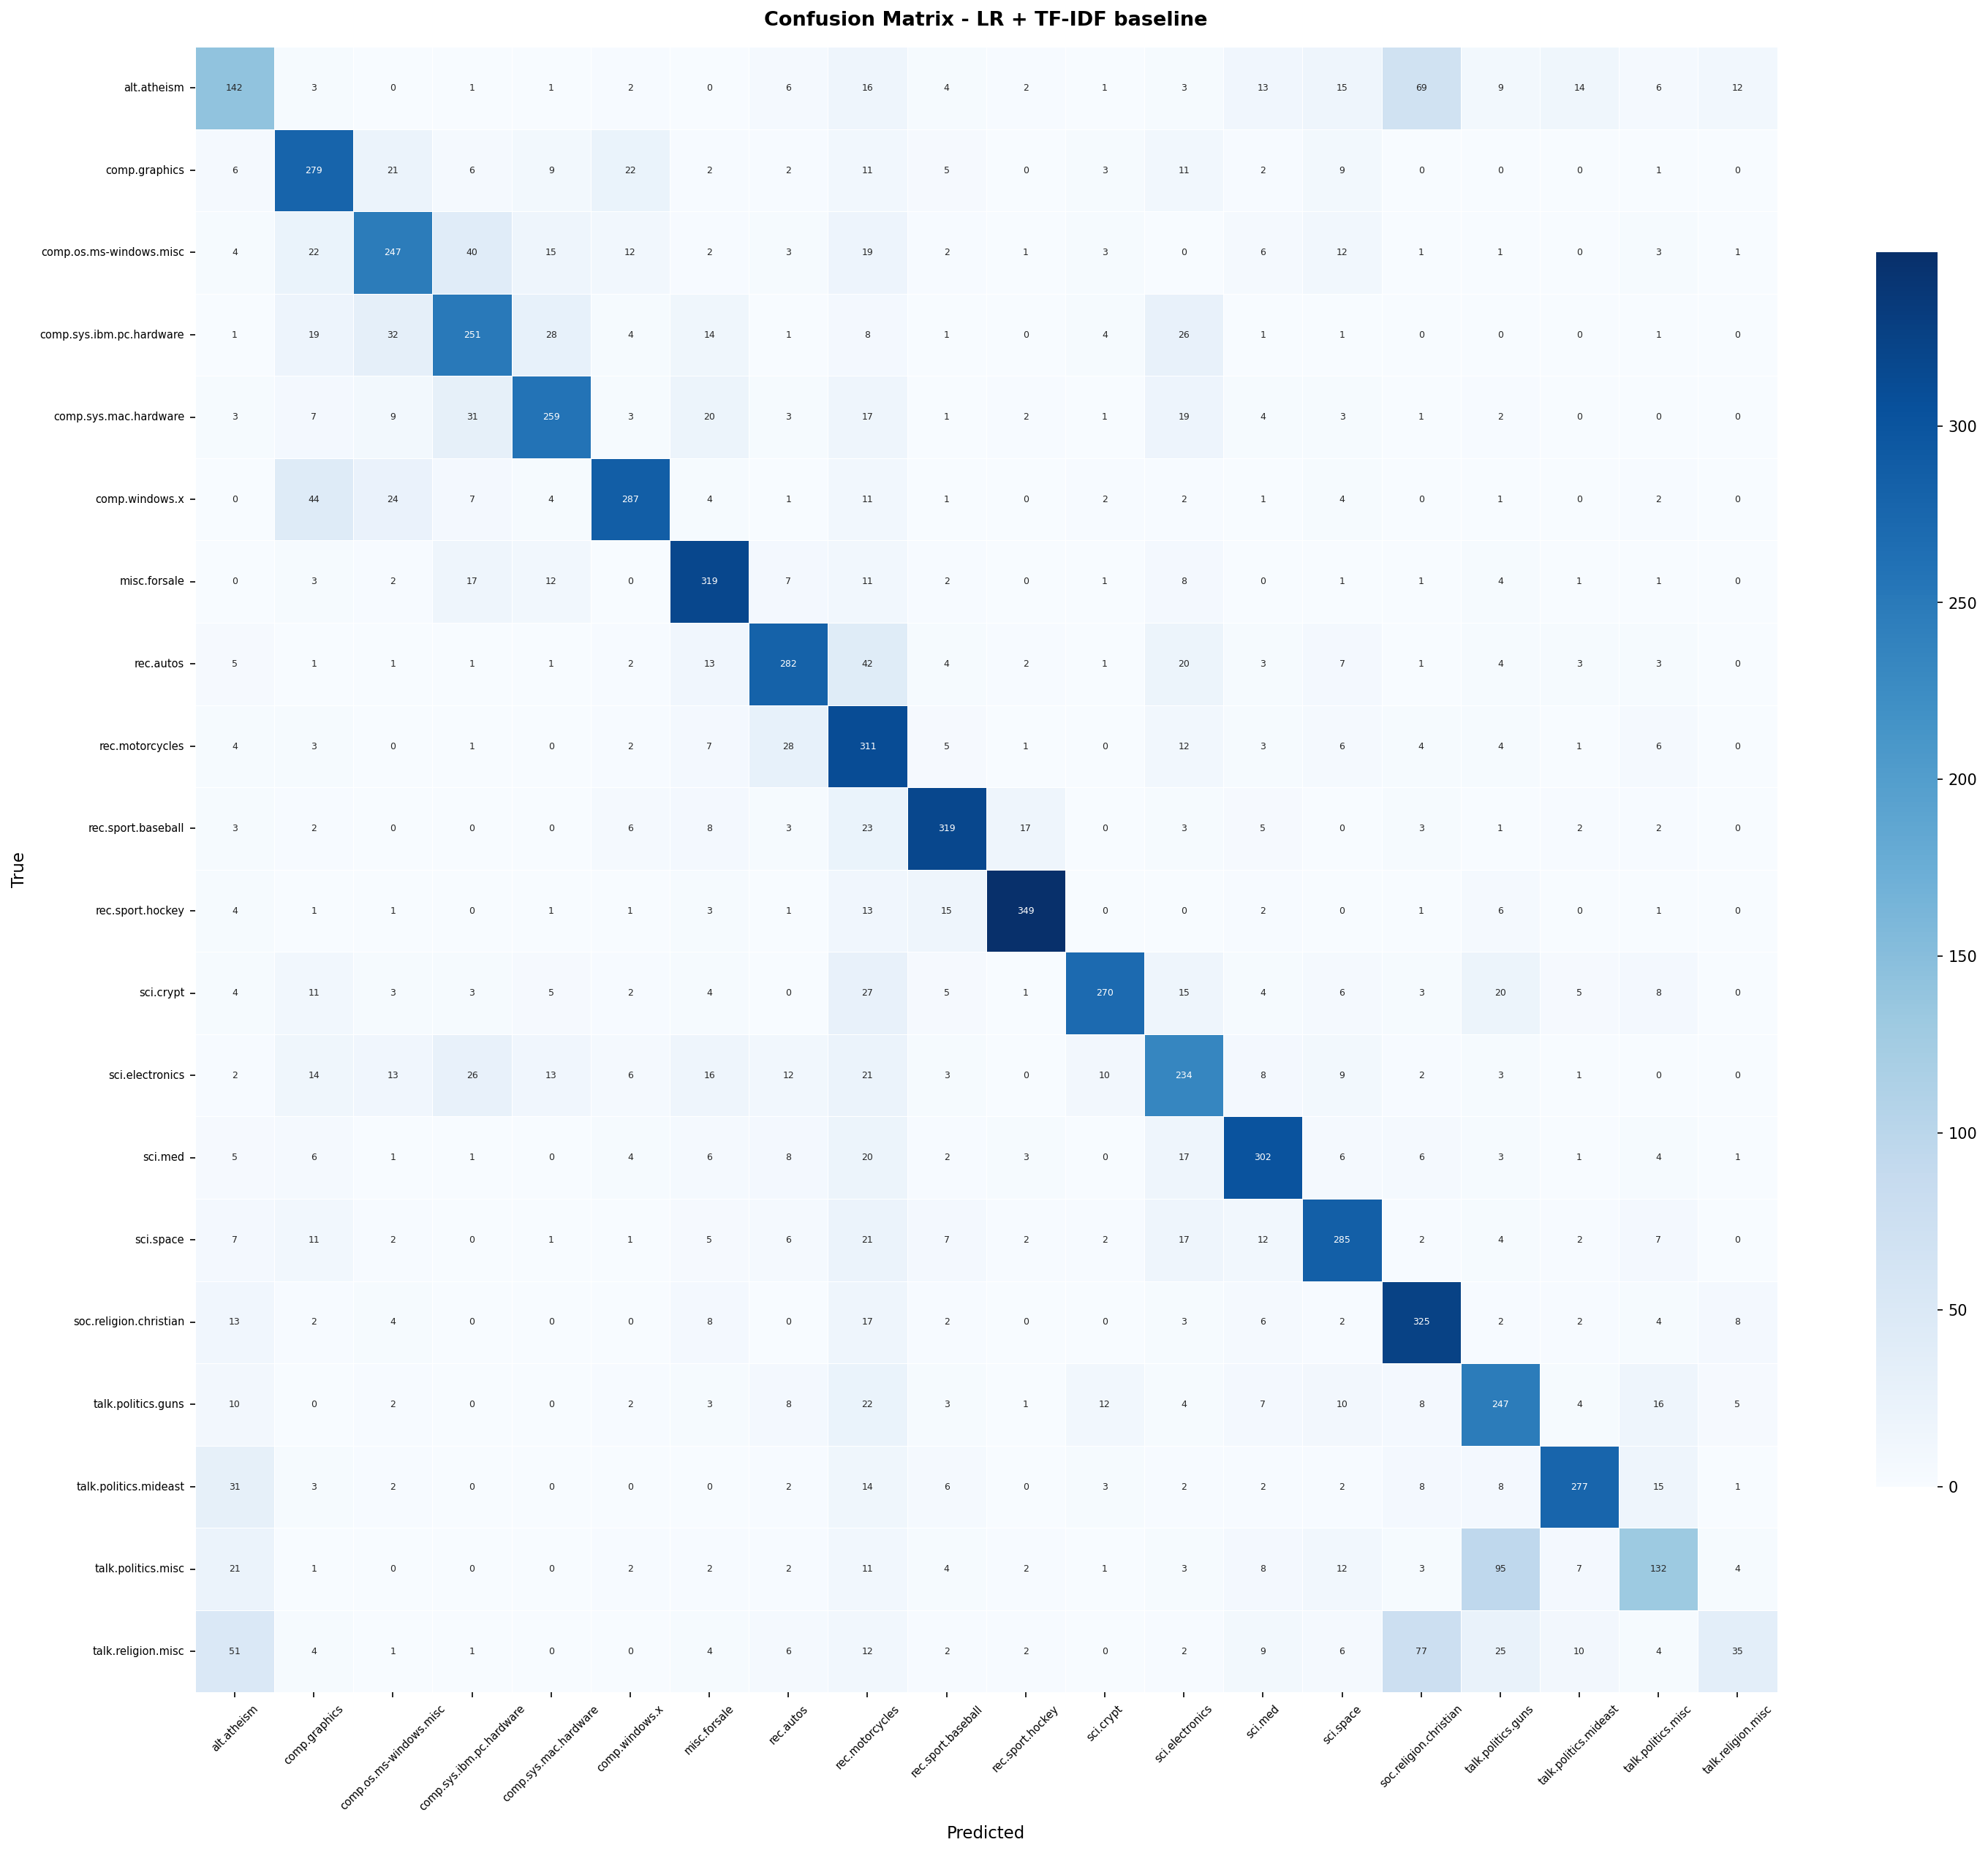
\includegraphics[width=\columnwidth]{figures/confusion_lr_baseline.png}%
  }{%
    \fbox{\parbox[c][0.22\textheight][c]{0.95\columnwidth}{\centering Missing figure:\\ \texttt{figures/confusion\_lr\_baseline.png}}}%
  }
  \caption{Confusion matrix -- LR + TF-IDF trained baseline.
    Confusion is strongest within related sub-domains such as
    \texttt{comp.*}, religion, and politics categories.}
  \label{fig:confusion-lr}
\end{figure}

\begin{figure}[t]
  \IfFileExists{figures/confusion_model1.png}{%
    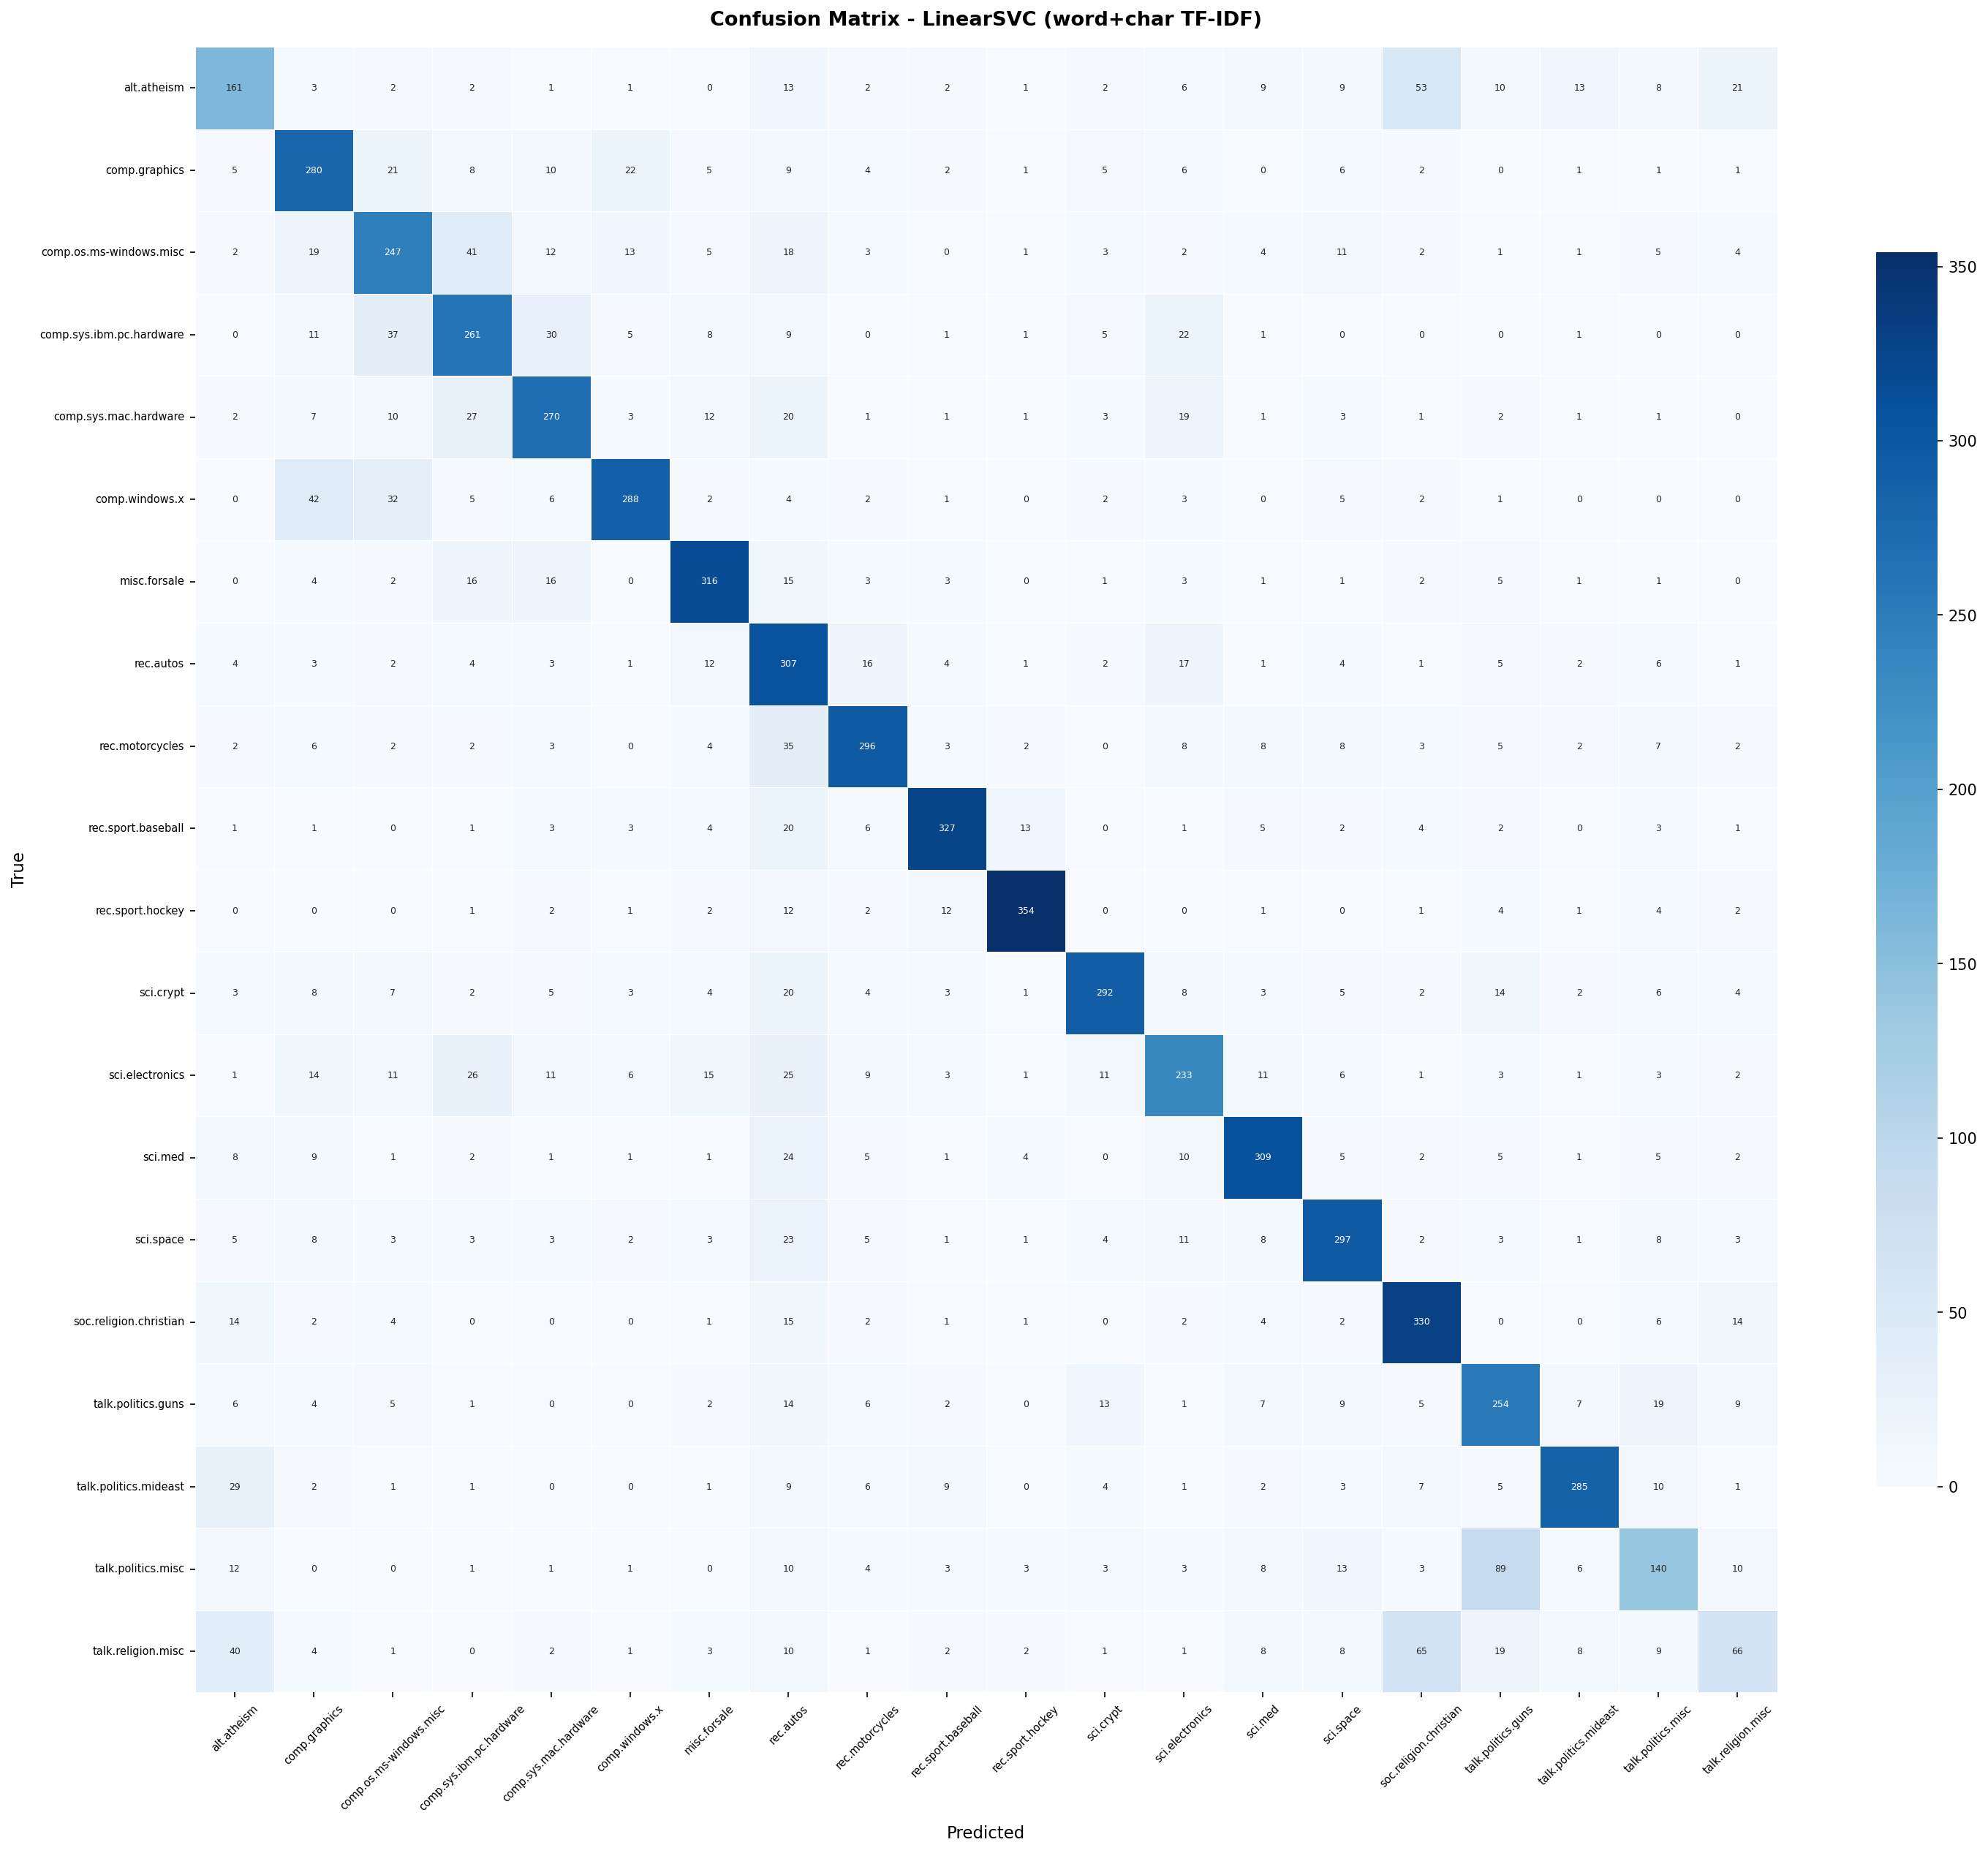
\includegraphics[width=\columnwidth]{figures/confusion_model1.png}%
  }{%
    \fbox{\parbox[c][0.22\textheight][c]{0.95\columnwidth}{\centering Missing figure:\\ \texttt{figures/confusion\_model1.png}}}%
  }
  \caption{Confusion matrix -- Multi-TF-IDF + LinearSVC (M1).
    Off-diagonal mass concentrates in the \texttt{comp.*} sub-cluster
    and the religion/politics overlap.}
  \label{fig:confusion-m1}
\end{figure}

\begin{figure}[t]
  \IfFileExists{figures/confusion_model2.png}{%
    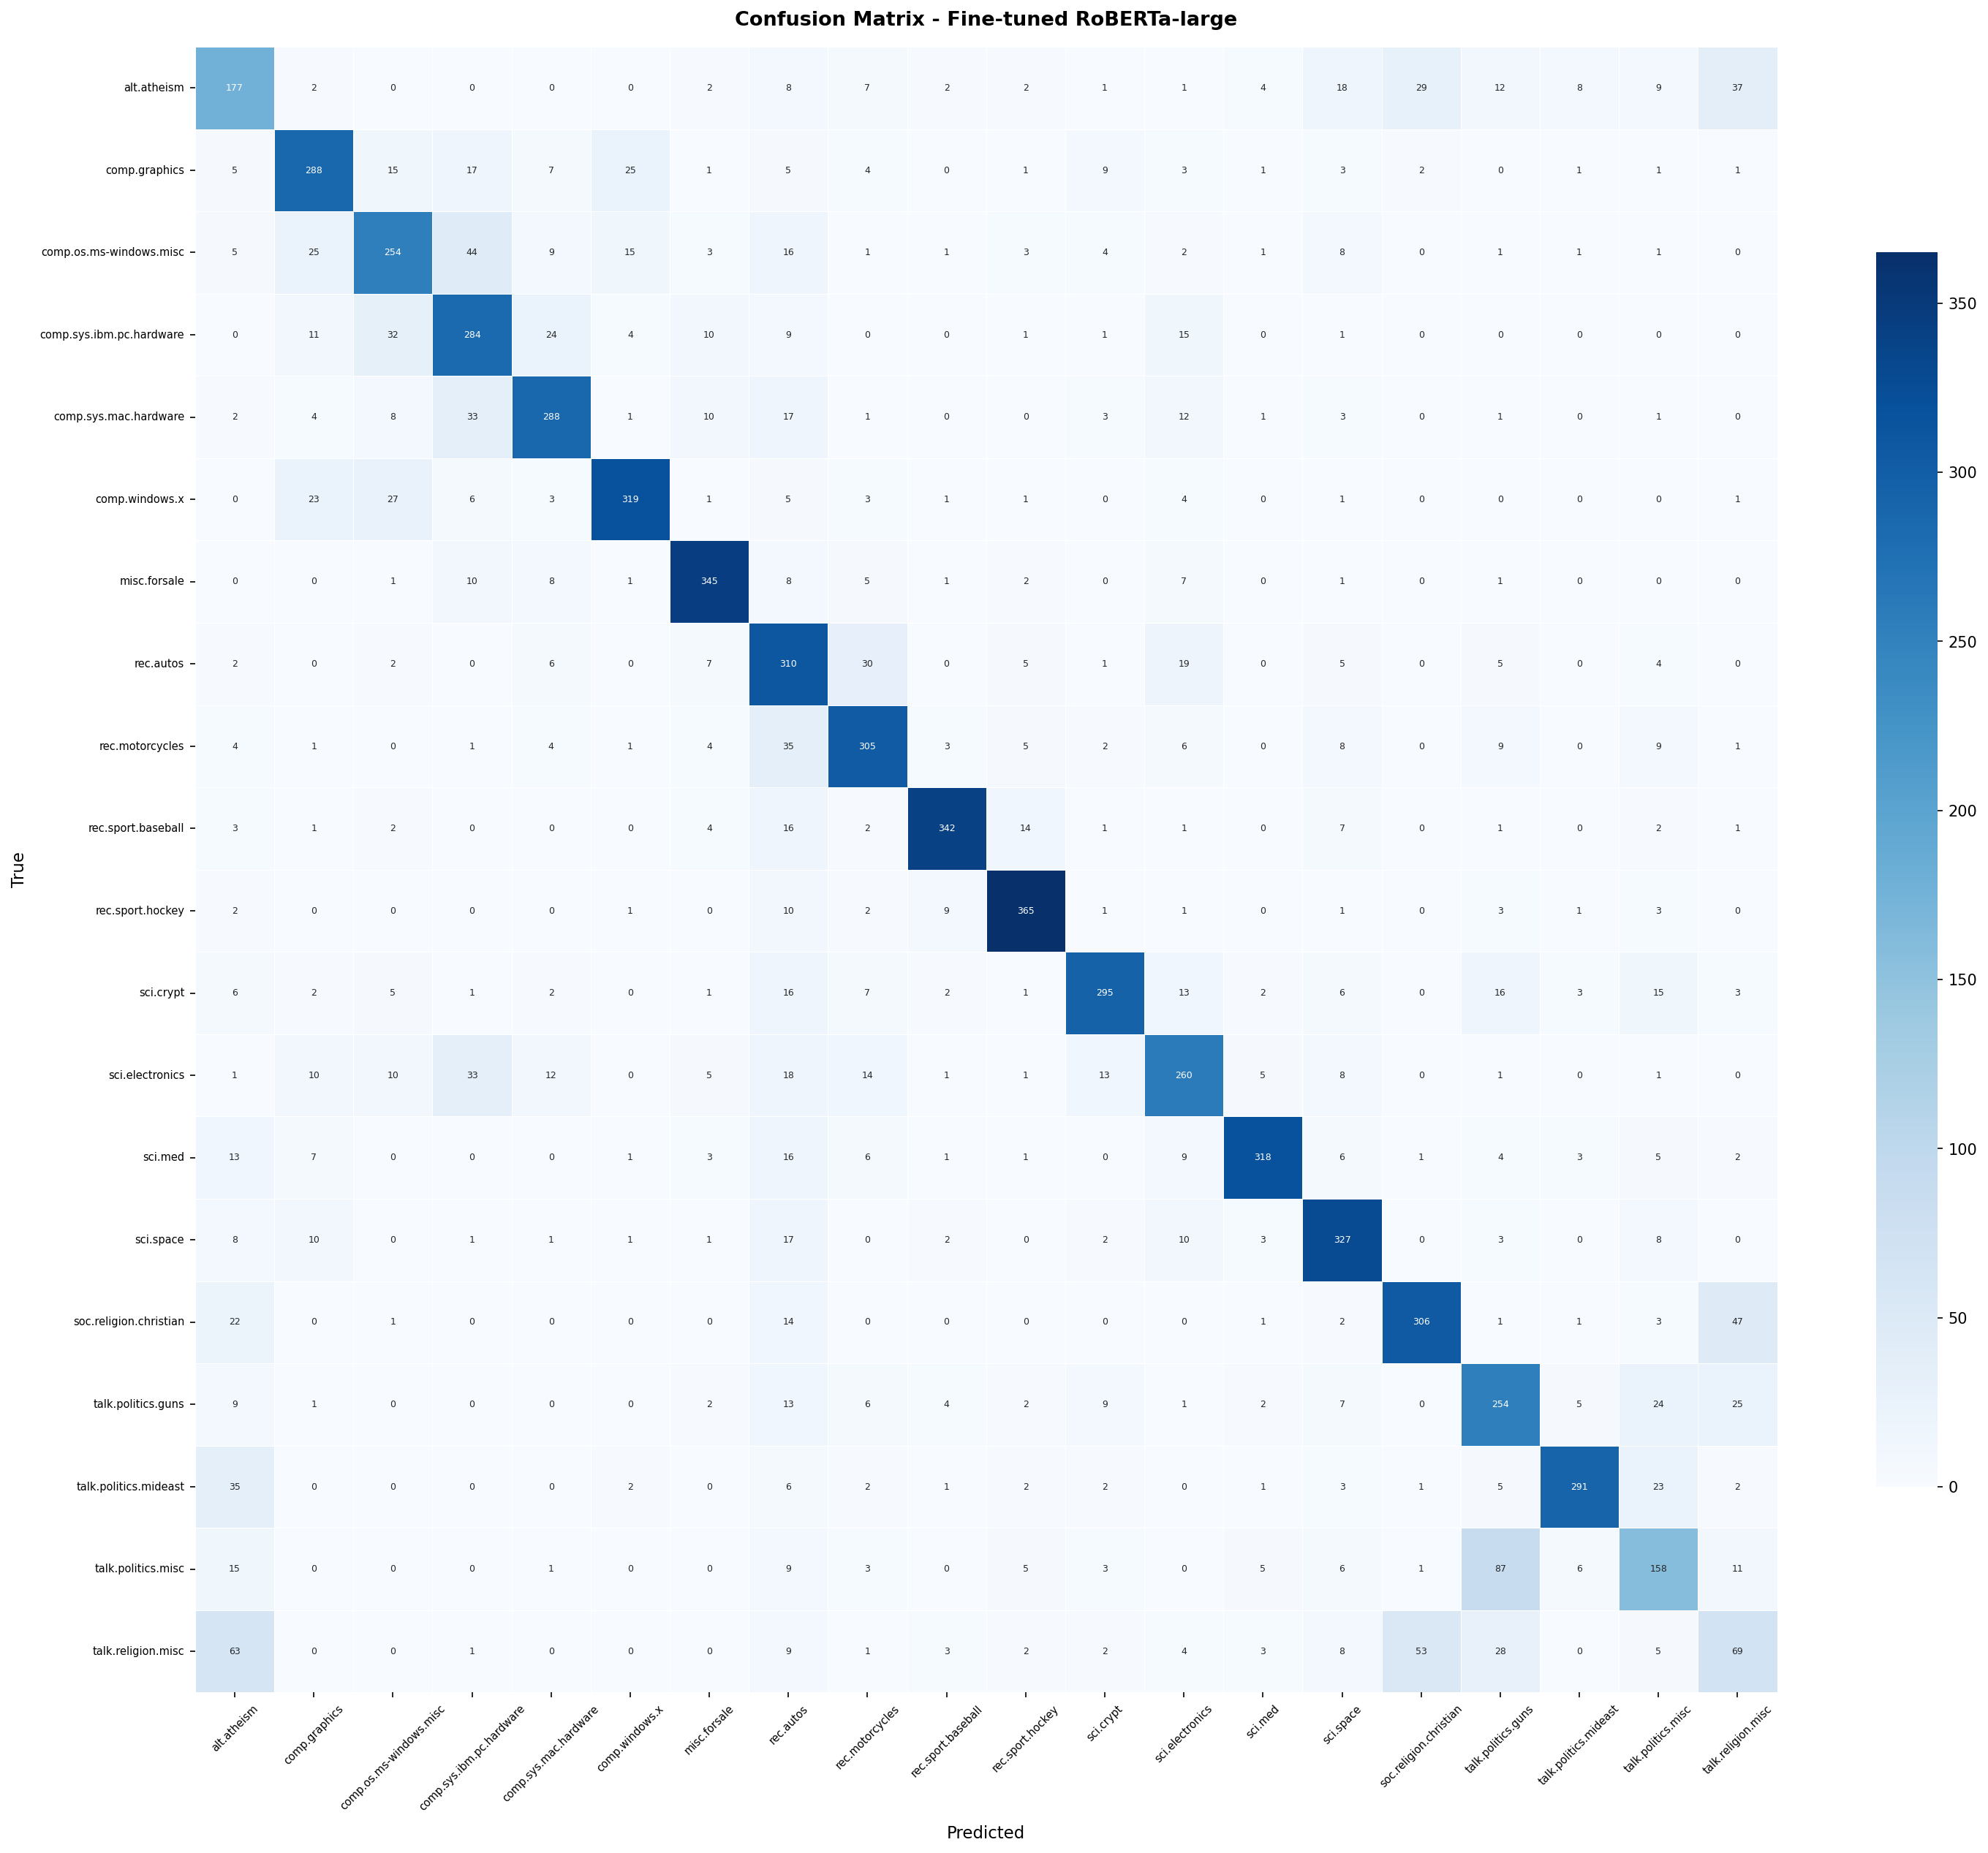
\includegraphics[width=\columnwidth]{figures/confusion_model2.png}%
  }{%
    \fbox{\parbox[c][0.22\textheight][c]{0.95\columnwidth}{\centering Missing figure:\\ \texttt{figures/confusion\_model2.png}}}%
  }
  \caption{Confusion matrix -- Fine-tuned RoBERTa-large (M2).
    Compared with M1 and the LR baseline, off-diagonal mass is reduced
    in several closely related class pairs.}
  \label{fig:confusion-m2}
\end{figure}

\begin{figure}[t]
  \IfFileExists{figures/confusion_model3.png}{%
    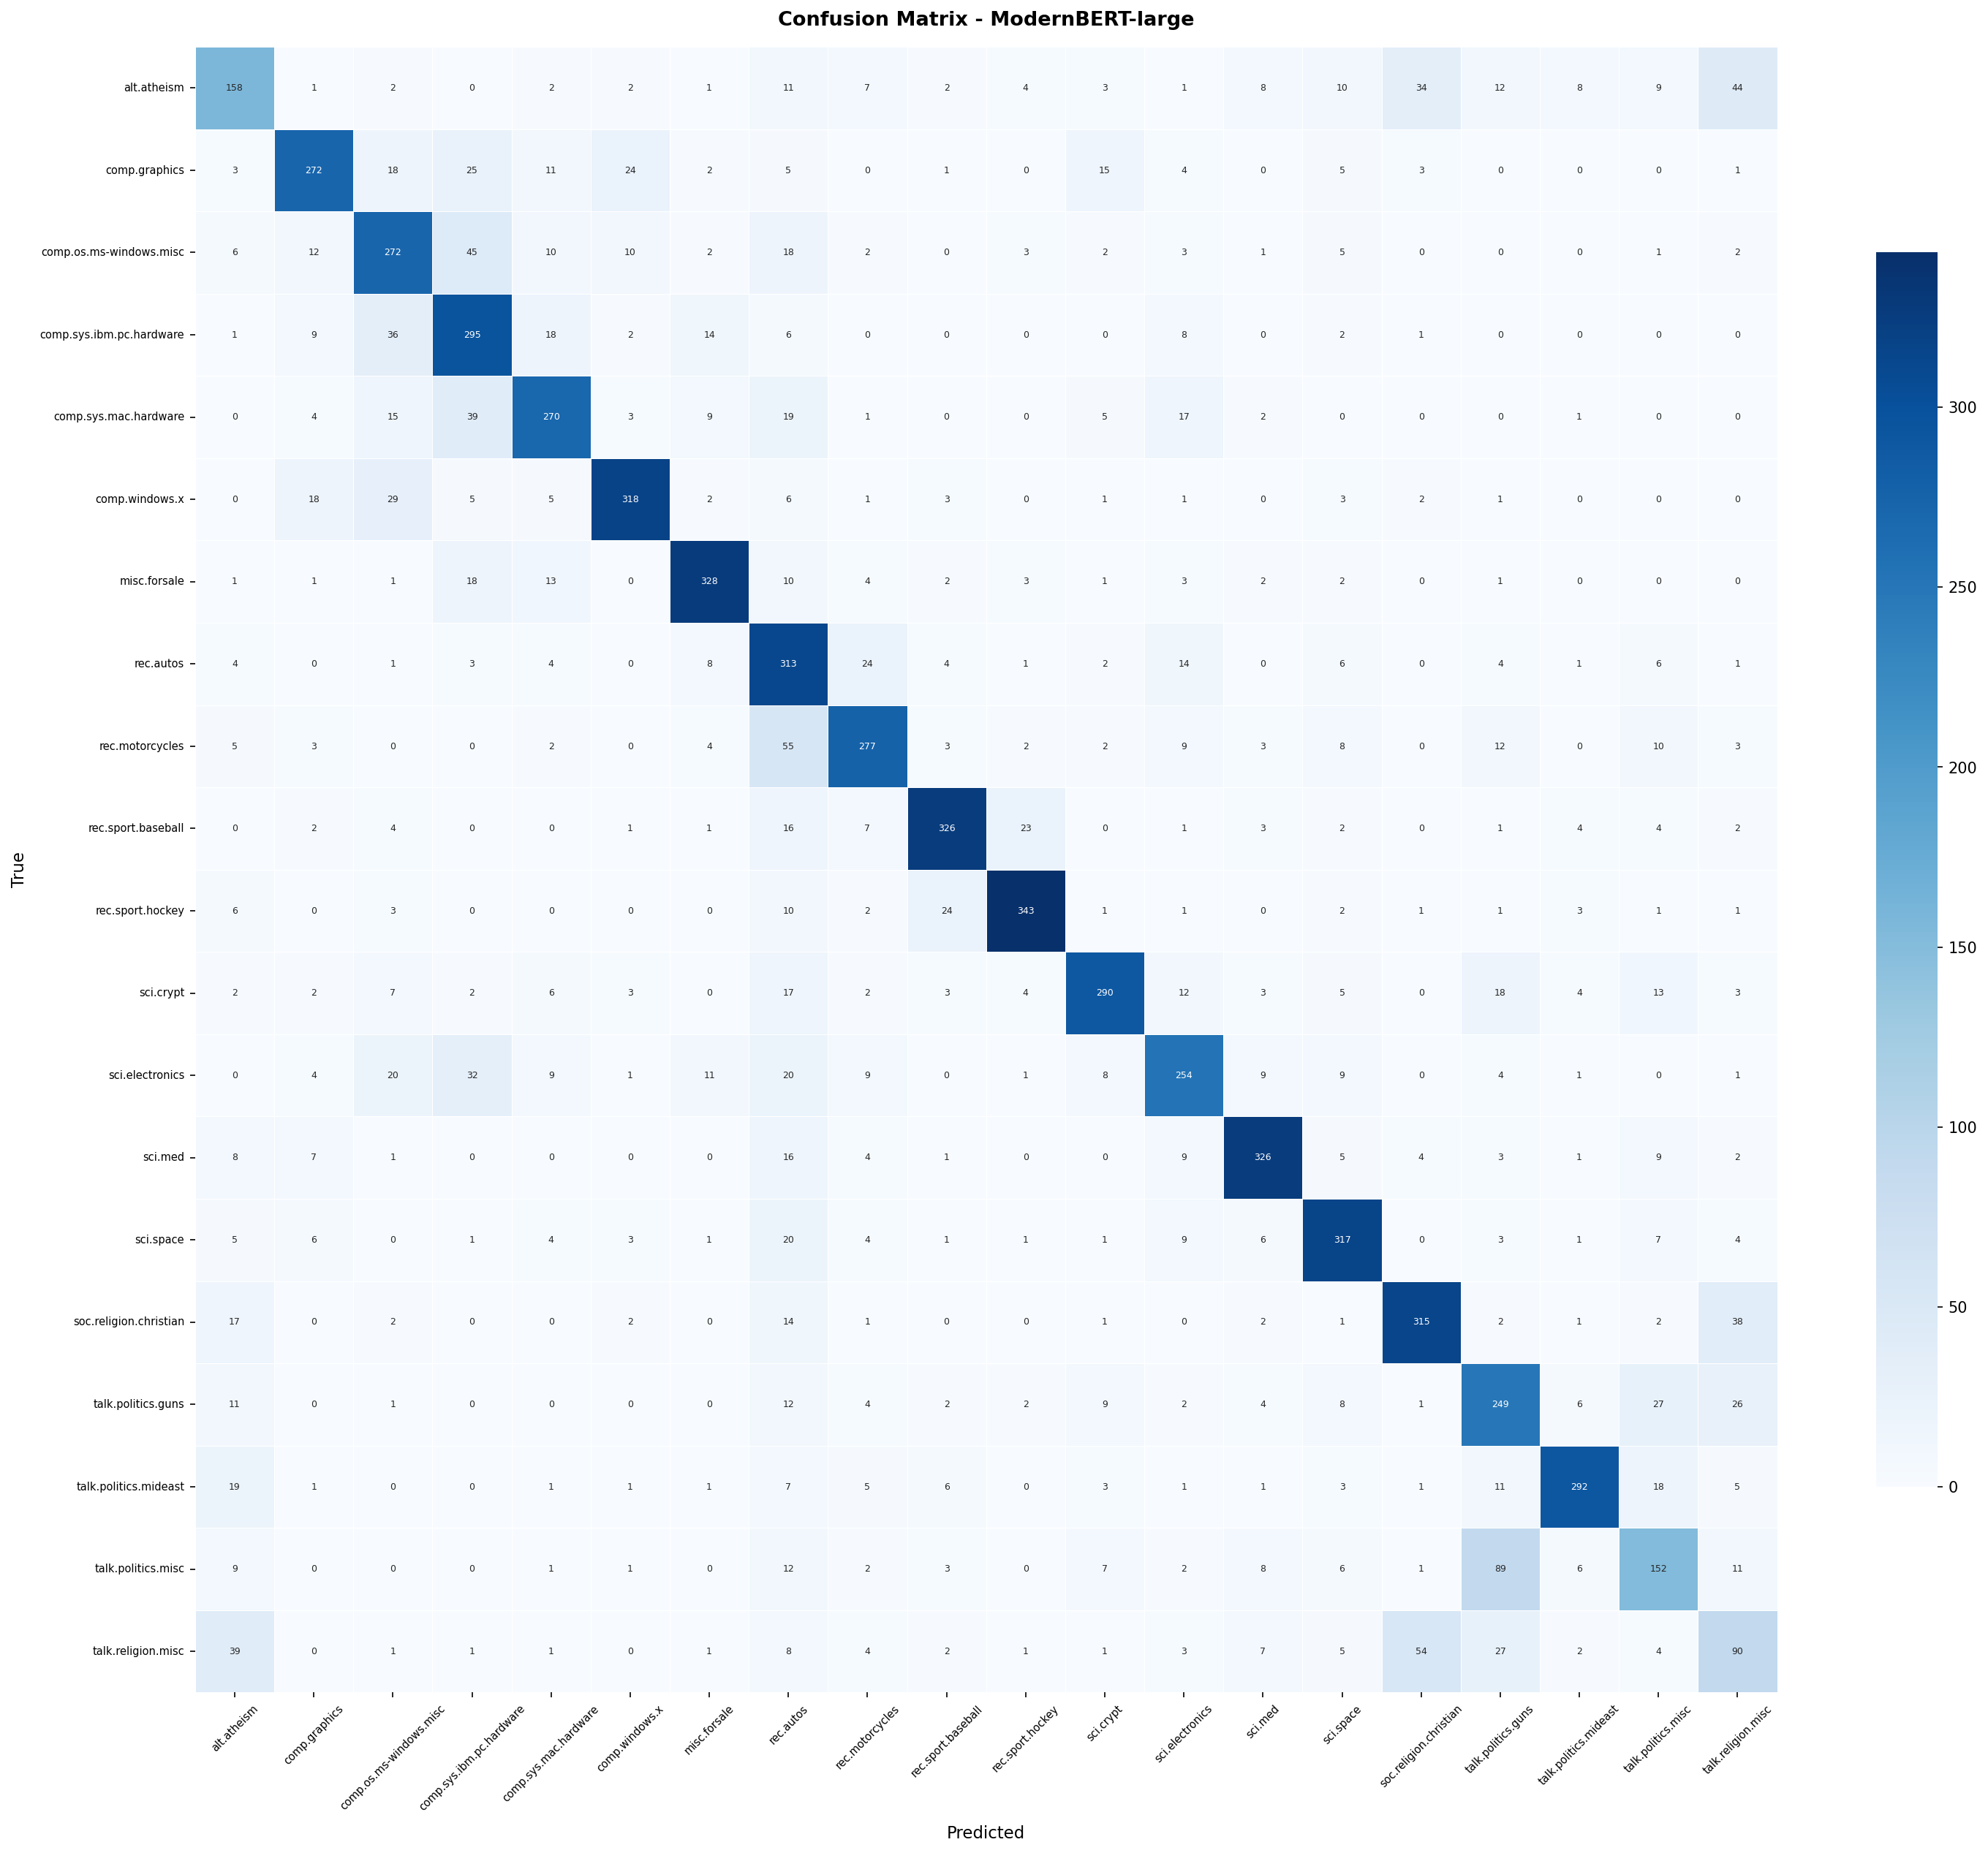
\includegraphics[width=\columnwidth]{figures/confusion_model3.png}%
  }{%
    \fbox{\parbox[c][0.22\textheight][c]{0.95\columnwidth}{\centering Missing figure:\\ \texttt{figures/confusion\_model3.png}}}%
  }
  \caption{Confusion matrix -- ModernBERT-large (M3).  Contextual
    representations reduce confusion in related categories compared
    to M1.}
  \label{fig:confusion-m3}
\end{figure}

Easy categories share distinctive vocabulary (\texttt{rec.sport.hockey},
$F1 \approx 0.90$; \texttt{misc.forsale}, $F1 \approx 0.80$).  Persistent
failures across all models are: (1)
\texttt{comp.sys.ibm.pc.hardware} $\leftrightarrow$
\texttt{comp.sys.mac.hardware}, hardware posts use identical vocabulary
when the platform name is absent; (2) the three religion groups, where
the distinction is stance rather than topic, even M2 and M3 reach only
$F1 \approx 0.87$ there versus $0.96$--$0.97$ for sports; (3) the
politics sub-groups, where single posts regularly span multiple topics.
M3's main improvement over M1 is on very short documents: on posts
reduced to $\leq$10 words after stripping ($\approx$4\% of test),
M1 achieves $\approx$60\% accuracy while M3 reaches $\approx$78\%.

\subsection{Recommendations}

The most promising next steps are: (1) \textbf{hierarchical
classification}, classify into 5 super-categories first, then handle
fine-grained sub-categories, isolating the religion confusion to a
dedicated 3-way classifier; (2) \textbf{targeted augmentation} for
religion and politics (back-translation or paraphrasing to vary stance
while holding topic constant); and (3) an \textbf{M1+M2 ensemble},
since their error profiles are largely complementary.

% ─────────────────────────────────────────────────────────────────
\section{Conclusions}
% ─────────────────────────────────────────────────────────────────

We built three classifiers on 20 Newsgroups ranging from a no-GPU
feature-engineering pipeline to a modern long-context encoder on two
H100s.  M1 (TF-IDF + LinearSVC) reaches 70.5\% test accuracy; M2
(RoBERTa-large) is our best at 73.75\% (F1 0.726) after fixing a
cluster-side LayerNorm checkpoint bug; M3 (ModernBERT-large) reaches
72.45\% (F1 0.715) after resolving a gradient-checkpointing
incompatibility with Flash Attention~2 (\texttt{use\_reentrant=False}).
All three beat the next-best clean-data classmate result of 72.2\%
(cruza7 BERT-base), confirming that careful preprocessing and
model-specific engineering matter at least as much as architecture
choice.

zhongx22's 82.3\% DistilBERT figure is not a fair comparison: it is a
validation-set score from data loaded without
\texttt{remove=('headers','footers','quotes')}, leaving category names
in document headers and making the task nearly trivial.

Residual errors concentrate in stance-defined categories (religion,
politics sub-groups), where a hierarchical classifier or an M1--M2
ensemble are the most promising paths forward.

% ─────────────────────────────────────────────────────────────────
\section*{Team Contributions}
% ─────────────────────────────────────────────────────────────────

\textbf{Abdul-Hadi Siddiqui} designed and implemented Model~1,
conducted the feature-engineering ablation, and led dataset
preprocessing, and wrote
and edited the final report.

\textbf{Eduardo Salvacion} designed and implemented Model~2, diagnosed
and fixed the LayerNorm cache bug, developed head+tail tokenisation,
wrote the GPU memory cleanup between models, built the evaluation
and error-analysis framework, and wrote
and edited the final report.

\textbf{Viransh Shah} designed and implemented Model~3, built the
multi-GPU training setup and \texttt{\_auto\_select\_gpus}, diagnosed
and fixed the FA2 gradient-checkpointing incompatibility, and wrote
and edited the final report.

% ─────────────────────────────────────────────────────────────────
\bibliography{custom}
% ─────────────────────────────────────────────────────────────────

\end{document}
